\documentclass[openany,overnay,a4paper, twoside, 14pt]{book}
\usepackage{graphicx}
\usepackage[utf8]{inputenc}
\usepackage[noindentafter]{titlesec}
\usepackage{wrapfig}
\usepackage[document]{ragged2e} %para poder justificar el texto
\usepackage[a4paper,width=150mm,top=25mm,bottom=25mm,bindingoffset=10mm]{geometry} %igualar los margenes de las paginas pares e impares
\usepackage[utf8]{inputenc}
\usepackage{hyperref}
\usepackage{listings}
\usepackage{xcolor}
\renewcommand{\contentsname}{Índice} %Cambio el nombre de Content a Índice
\title{\Huge Test de Usuarios - CaixaBank.es\\}
%Añado la imagen justo antes en el titulo
\author{
    Herrero Pina, María\\
    IES Ítaca\\
    0024mherrero@e-itaca.es\\
\date{February 2022}}
\pagestyle{plain} %Para que los números de página aparezcan siempre en medio
\begin{document}
\maketitle
\newpage
\tableofcontents
\rmfamily
\justify
\setcounter{chapter}{1}
\chapter*{Introducción}
\addcontentsline{toc}{chapter}{Introducción}
Se entiende por test de usuario, una prueba que nos permite recoger información cualitativa para entender, cómo y por qué los usuarios utilizan un producto.\\Durante la realización del test se pide a los usuarios realizar una serie de tareas para interactuar con el producto, de forma que averiguamos:
\begin{itemize}
    \item Cómo navegan estos por la página web.
    \item Por qué llevan a cabo ciertas acciones.
    \item Qué valoran positivamente.
    \item Qué funciones echan en falta.
\end{itemize}
Gracias a este test se podrá mejorar el producto y así conseguir mejorar la experiencia del usuario.
En este trabajo, se va a llevar a cabo un test de usuarios, mediante un modelo ya proporcionado. Para la realización de este trabajo hemos seleccionado la página web que nos proporciona CaixaBank. Una vez realizado este test, sacaremos unas conclusiones acerca de los resultados obtenidos.
\chapter*{Identidad}
\addcontentsline{toc}{chapter}{Identidad}
\textbf{\textcolor{red}{1.- }¿Con la información que se ofrece en pantalla, es posible saber a qué institución o empresa corresponde el sitio? ¿Cómo lo sabe?}\\
\textcolor{blue}{Se conoce la institución perfectamente, dado que su nombre aparece al principio de la página web.}\\
\\
\textbf{\textcolor{red}{2.-} ¿Hay algún elemento gráfico o de texto que le haya ayudado a entender más claramente a que institución o empresa pertenece el sitio?}\\
\textcolor{blue}{Si, porque aparece el logo y el nombre de dicha institución al inicio de la página web.}\\
\\
\textbf{\textcolor{red}{3.-} <Sólo si no fue mencionado antes> ¿Relaciona los colores predominantes en el sitio web con la institución? ¿Relaciona la dirección del sitio web con la institución?}\\
\textcolor{blue}{Los colores predominantes no están relacionados con el logo de la empresa.}\\
\\
\textbf{\textcolor{red}{4.-} <Sólo si no fue mencionado antes> ¿De los elementos que muestra esta pantalla, hay algo que usted crea que está fuera de lugar, porque no pertenece a la institución o empresa que usted identifica como propietaria?}\\
\textcolor{blue}{No.}\\
\\
\textbf{\textcolor{red}{5.-} ¿Distingue alguna imagen que represente (logotipo) a la institución? ¿Cree que aparece en un lugar importante dentro de la página? ¿Puede leer el nombre de la institución? ¿Es claro?}\\
\textcolor{blue}{Si que aparece el logo, está al principio de la página web. Si que aparece el nombre de la institución y además está claro.}\\
\\
\textbf{}{\textcolor{red}{6.-} ¿Hacia qué tipo de audiencia cree usted que está dirigido este sitio? ¿Por qué?}\\
\textcolor{blue}{Va dirigido a cualquier persona que tenga o quiera tener en un futuro una cuenta bancaria en CaixaBank. Esta información se deduce de qué en la página inicial te deja elegir entre varias opciones o accesos: Familias, Banco Premier, Banca Privada, Empresas, Negocios... }\\
\\
\textbf{\textcolor{red}{7.-} Si tuviera que tomar contacto telefónico o enviar una carta tradicional a la institución o empresa propietaria del sitio web, ¿se ofrece información de números o direcciones? ¿Son útiles como para hacer esa tarea? ¿Le costó encontrar esa información?}\\
\textcolor{blue}{Si, se ofrece el número de teléfono, un formulario de contacto o redes sociales. Si que pareen útiles. No.}
\chapter*{Contenido}
\addcontentsline{toc}{chapter}{Contenido}
\textbf{\textcolor{red}{1.-} ¿Le parece adecuada la selección de contenidos destacados en la portada o usted echó de menos otras áreas de información que le habría gustado ver destacadas?}\\
\textcolor{blue}{No me he sentido cómoda con la selección de contenidos de la portada, ya que, lo que únicamente aparece, son premios y regalos que se pueden financiar con la institución.}\\
\\
\textbf{\textcolor{red}{2.-} ¿Al ver la portada del sitio, pudo distinguir de una sola mirada cuál era el contenido más relevante que se ofrecía? ¿Cómo logró hacer esa distinción? }\\
\textcolor{blue}{El contenido más relevante son ofertas de financiación de bienes muebles e inmuebles con la institución. Es lo que más destaca de la página web, ya que aparece al inicio de esta.}\\
\\
\textbf{\textcolor{red}{3.-} ¿Es fácil distinguir los nuevos contenidos que presenta el sitio web? ¿Por ejemplo, es posible saber cuándo fue la última actualización del sitio?}\\
\textcolor{blue}{No, en ninguna parte aparece cuando se realizó la última actualización de la página.}\\
\\
\textbf{\textcolor{red}{4.-} ¿Los textos usados en los contenidos de los enlaces son suficientemente descriptivos de lo que se ofrece en las páginas hacia las cuales se accede a través de ellos?}\\
\textcolor{blue}{Si, además aparecen muchos en "Negrita" (Bold).}\\
\\
\textbf{\textcolor{red}{5.-} ¿En caso de que los contenidos ofrecieran archivos adjuntos, fue fácil saber su peso o si eran de un formato diferente al de una página web? ¿Le ayudó la información ofrecida por el sitio sobre dichos archivos? ¿O no recibió ninguna información? }\\
\textcolor{blue}{No hay archivos adjuntos, por lo qué no podría responder a la pregunta.}\\
\\
\textbf{\textcolor{red}{6.-} En caso de haber información relacionada con la que estaba viendo, ¿se le ofreció de manera simple? ¿O tuvo que volver a navegar para encontrarla?}\\
\textcolor{blue}{No aparece información similar a la que estaba viendo anteriormente.}\\

\chapter*{Navegación}
\addcontentsline{toc}{chapter}{Navegación}
\textbf{\textcolor{red}{1.-} ¿Puede ver en la portada y las demás páginas, la forma en que se navega por el sitio? ¿ Se distingue fácilmente?}\\
\textcolor{blue}{Si, se seguir la página web de forma intuitiva.}\\
\\
\textbf{\textcolor{red}{2.- }¿Existen elementos dentro de las páginas, que le permitan saber exactamente dónde se encuentra dentro de este sitio y cómo volver atrás sin usar los botones del programa navegador? }\\
\textcolor{blue}{Es fácil entrar en el sitio, pero no existen ese tipo de elementos.}\\
\\
\textbf{\textcolor{red}{3.-} ¿Cómo vuelve desde cualquier página del sitio a la página de inicio? ¿Ve alguna forma de hacerlo, que no sea presionando el botón del buscador? ¿Le parece claro?}\\
\textcolor{blue}{Para volver a la página de inicio, simplemente hay que realizar clic en el logo o nombre de la institución que aparece arriba del todo de la página web. Si está claro, ya que, es el mismo método que se utiliza en otras páginas web.}\\
\\
\textbf{\textcolor{red}{4.-} ¿Habitualmente, cómo logra acceder directamente a los contenidos sin tener que navegar? ¿Usa el buscador? ¿Usa el Mapa del Sitio? ¿Los puede ver en este sitio? ¿Echa de menos alguno?}\\
\textcolor{blue}{Lo que realizo habitualmente es buscar el buscador y ahí se puede escribir lo que se quiere encontrar. En pocas ocasiones uso el mapa del sitio. De está página web no echo en falta nada.}\\
\\
\textbf{\textcolor{red}{5.-} ¿Logra distinguir gráficamente los enlaces visitados de aquellos que no ha visitado aún? <Si existe esa diferencia de colores>¿Le ayuda esa diferencia?}\\
\textcolor{blue}{En esta página no hay distinción de ese tipo, aunque si que ayudaría.}\\
\\
\textbf{\textcolor{red}{6.-} El sitio tiene varios niveles de navegación y Usted ha ingresado y salido de varios de ellos. ¿La información que se le ofrece en pantalla le parece adecuada para entender dónde está ubicado en cualquier momento? ¿Se ha sentido perdido dentro del sitio? ¿Si lo ha sentido, recuerda en qué área fue? ¿Si no lo ha sentido, qué elemento del sitio cree que le ayudó más a orientarse?}\\
\textcolor{blue}{Resulta complicado saber exactamente donde estas, porqué sabes a donde te has metido, porqué aparece como título de la página web, pero no sabes en que parte exacta estas de la página.}\\
\\

\chapter*{Gráfica Web}
\addcontentsline{toc}{chapter}{Gráfica Web}
\textbf{\textcolor{red}{1.-} ¿Le pareció adecuada la forma en que se muestran las imágenes en el sitio web? ¿Son nítidas? ¿Son adecuadas para representar el contenido del que trata el sitio?}\\
\textcolor{blue}{Si que son nítidas y también informan de que trata cada apartado del sitio.}\\
\\
\textbf{\textcolor{red}{2.-} ¿Las imágenes grandes se demoraron más de lo esperado? ¿Tuvo que seguir navegando sin que llegaran a mostrarse completamente? ¿Cree que el sitio es muy lento?}\\
\textcolor{blue}{Apenas se nota diferencia entre las imágenes de gran tamaño y las de menor.}\\
\\
\textbf{\textcolor{red}{3.-} ¿Se fijó si el sitio tenía gráficas con animaciones? ¿Hay alguna que le haya llamado la
atención? ¿Ninguna?}\\
\textcolor{blue}{Si que aparecen animaciones al pasar el ratón por encima de una sección.}\\
\\
\textbf{\textcolor{red}{4.-} ¿Considera que gráficamente el sitio está equilibrado, muy simple o recargado?}\\
\textcolor{blue}{Creo que está muy simple.}\\
\\
\textbf{\textcolor{red}{5.-}¿Recuerda si el sitio tenía banners (avisos) publicitarios? ¿Tuvo intención o llegó a hacer clic sobre alguno? ¿Por qué le hizo clic? ¿Qué le llamó la atención? }\\
\textcolor{blue}{No ha aparecido ningún tipo de banner.}\\
\\
\chapter*{Búsqueda}
\addcontentsline{toc}{chapter}{Búsqueda}
\textbf{\textcolor{red}{1.-} ¿Utiliza normalmente un buscador al acceder a un sitio web? ¿Distinguió si en este sitio se ofrecía un buscador? ¿Dónde está?}\\
\textcolor{blue}{No, suelo usar el menú lateral que aporta la página web.}\\
\\
\textbf{\textcolor{red}{2.-} <antes de usar el buscador> ¿Cómo haría la operación de buscar? ¿Qué escribiría? ¿Dónde lo escribiría?}\\
\textcolor{blue}{Utilizaría la barra lateral. En le buscador externo a la página web buscaría lo que necesitará, poniendo al final el nombre de la instutución a la que me refiero.}\\
\\

\textbf{\textcolor{red}{3.-} <antes de presionar el botón Buscar > ¿Qué espera encontrar?
<al ver la página de resultados> ¿Ese es lo que esperaba encontrar?, ¿Le sirve?}\\
\textcolor{blue}{El resultado que me lleve a la página que le he indicado. Lo que he encontrado hace exactamente Lo dispuesto en la pregunta anterior.}

\chapter*{Feedback}
\addcontentsline{toc}{chapter}{Feedback}
\textbf{\textcolor{red}{1.-} ¿Encuentra alguna forma online y offline de ponerse en contacto con la empresa o institución, para hacer sugerencias o comentarios? <ver pregunta similar en la parte de Identidad>}\\
\textcolor{blue}{Si, como he dicho en la otra parte del test, se encuentra un número de teléfono, un formulario de contacto o redes sociales.}\\
\\
\textbf{\textcolor{red}{2.-} <Tras la operación de enviar algún formulario vía web> ¿Al mandar datos mediante un formulario, el web le avisa si los recibió correctamente o no?}\\
\textcolor{blue}{Si que avisa de que se envió correctamente.}

\chapter*{Utilidad}
\addcontentsline{toc}{chapter}{Utilidad}
\textbf{\textcolor{red}{1.-} ¿Tras una primera mirada, le queda claro cuál es el objetivo del sitio? ¿Qué contenidos y servicios ofrece? ¿Los puede enumerar? }\\
\textcolor{blue}{El objetivo de la página web, es ver que productos ofrece la institución, tanto para familias, empresas, negocios...}\\
\\
\textbf{\textcolor{red}{2.-} ¿Cree que los contenidos y servicios que se ofrecen en este sitio son de utilidad para su caso personal?}\\
\textcolor{blue}{Personalmente, no hago uso de esta página web de forma habitual, pero en un principio si que cumple con su objetivo.}\\
\\
\textbf{\textcolor{red}{3.-} ¿Qué es lo que más te llamó la atención positivamente o negativamente de la utilidad que ofrece el sitio web?}\\
\textcolor{blue}{Lo que más me ha llamado la atención es que no aparezca cuando entras en una sección, un menú o algún botón para volver atrás.}

\chapter*{Conclusiones}
\addcontentsline{toc}{chapter}{Conclusiones}
Después de la realización de este test de usuario acerca de la página web de CaixaBank, hemos obtenido estos resultados:
\begin{figure}[h]
\centering

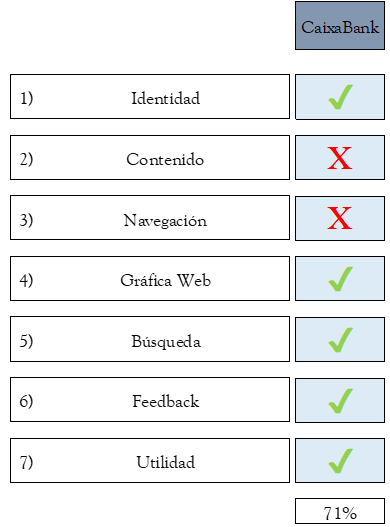
\includegraphics[scale = 0.7]{taba_resumen_caixa.png}
\renewcommand{\figurename}{Tabla resumen}
\renewcommand{\thefigure}{}
\caption{\textit{Test de Usuario}}
\renewcommand{\figurename}{Fuente}
\caption{Propia}
\end{figure}
\\
Por lo tanto, podemos concluir que la página web de CaixaBank se identifica genial, aunque su contenido y su navegación parecen escasas, por otro lado, su gráfica web es idónea, al igual que su búsqueda, feedback y su utilidad. Esto significará que lo único a modificar seria su contenido, en el sentido de hacer más visual otro tipo de contenido más importante que la página de por si ya lo tiene y el modo de navegación, sobre todo al entrar en una sección y no poder volver a atrás de forma intuitiva.


\end{document}
